Our security proof is based on the security proof of NIPoPoWs Suffix Security Proof
under a soft or hard fork. Keep in mind that we operate under the condition of
(1/3)-bounded adversary.\\

The notion of Chain Quality is decisive for the operation of NIPoPoWs under a
velvet fork. Before stepping into the security proof we remind its formal
definition\ref{defn:chain_quality} of this notion and the basic Theorem where its basic metric is computed.\\


\begin{thm}{\textbf{Chain Quality Parameter}}
	In a typical execution the chain quality property holds with parameter $\mu_{cq} > 1 - (1 + \frac{\delta}{2}) \cdot \frac{t}{n-t} - \frac{\delta}{2}$.
\end{thm}
\textit{Proof.} See \cite{Backbone}.\\

Our interest lies in keeping $\mu_{cq} \geq \dfrac{1}{2}$.
From Theorem 3 we have:
\begin{equation*}
	1 - (1 + \frac{\delta}{2}) \cdot \frac{t}{n-t} - \frac{\delta}{2} \geq \dfrac{1}{2} \Rightarrow 
	(1 + \delta)t \leq (1-\delta)(n-t)
\end{equation*}

Thus we have:
\begin{center}
\begin{equation}
	t \leq \dfrac{(1-\delta)}{2}(n - t)
\end{equation}
\end{center}

\begin{thm}{\textbf{Suffix Proofs Security under velvet fork}}
	Assuming honest majority under velvet fork conditions (\ref{defn:velvet_honest_majority}) such that $t \leq (1 - \delta) \dfrac{n_h}{2}$ where $n_h$ the number of upgraded honest players, the non-interactive proofs-of-proof-of-work construction for computable k-stable monotonic suffix-sensitive predicates under velvet fork conditions in a typical execution is secure.
\end{thm}
\textit{Proof.} By contradiction. We follow the proof construction of Theorem 2
and extend it. Let $Q$ be a k-stable monotonic suffix-sensitive chain
predicate. Assume NIPoPoWs under velvet fork on $Q$ is insecure. Then, during
an execution at some round  $r_3$, $Q(C)$ is defined and the verifier $V$
disagrees with some honest participant. Assume the execution is typical. $V$
communicates with adversary $A$ and honest prover $B$. The verifier receives
proofs $\pi_A, \pi_B$. Because $B$ is honest, $\pi_B$ is a proof constructed
based on underlying blockchain $C_B$ (with $\pi_B \subseteq C_B$), which $B$
has adopted during round $r_3$ at which $\pi_B$ was generated. Consider $\widetilde{C}_A$ the set of blocks defined as $\widetilde{C}_A = \pi_A \cup \{ (\forall b_A \in \pi_A, \exists h,r : b_A \in \mathcal{C}_{h}^{r}): C_h^r\{:b_A\} \}$, where $\mathcal{C}_h^r$ a chain that an honest player $p$ has adopted at some round $r$. Note that $\widetilde{\mathcal{C}}_A$ forms a chain considering the interlink pointers.
%Consider $\widetilde{C}_A$ the chain containing at least some of the blocks in $\pi_A$, while the remaining blocks $\pi_A$ must belong in $C_B$.

The verifier outputs $\neg Q(C_B)$. Thus it is necessary that $\pi_A \geq \pi_B$.
We show that $\pi_A \geq \pi_B$ is a negligible event.
Let $b = LCA(\pi_A, \pi_B)$. Let the levels of comparison decided by the verifier
be $\mu_A$ and $\mu_B$ respectively. Let $\mu'_B$ be the adequate level of proof
$\pi_B$  with respect to block $b$. Call $\alpha_A = \pi_A \uparrow^{\mu_A}\{b:\}$,
$\alpha'_B = \pi_B \uparrow^{\mu'_B}\{b:\}$.

%%%%%%%%   reconsider this paragraph
Our proof construction is based on the following scheme: we show that the competing
suffix proofs can be conceived as consisting of three distinct parts. Each part
denotes a specific round set and is named after the number of blocks existing
in $\pi_A$ for that round set. Part $k_1$ stands for the first part of each proof
between blocks $b = LCA(\pi_A, \pi_B)$ and $b_2 = LCA(\widetilde{\mathcal{C}}_A, C_B)$. Part $k_2$ stands for the second part
of the proofs considering the rounds from block $b_2$ and until
the Common Prefix is established at $\mathcal{C}_B$ for that fork point.
The third and last part, $k_3$ stands for the rest of the blocks in each proof.\\
The above are illustrated, among other, in Parts I, II of Figure \ref{fig:proof_velvet}.

\begin{figure}[h!]
	\begin{center}
		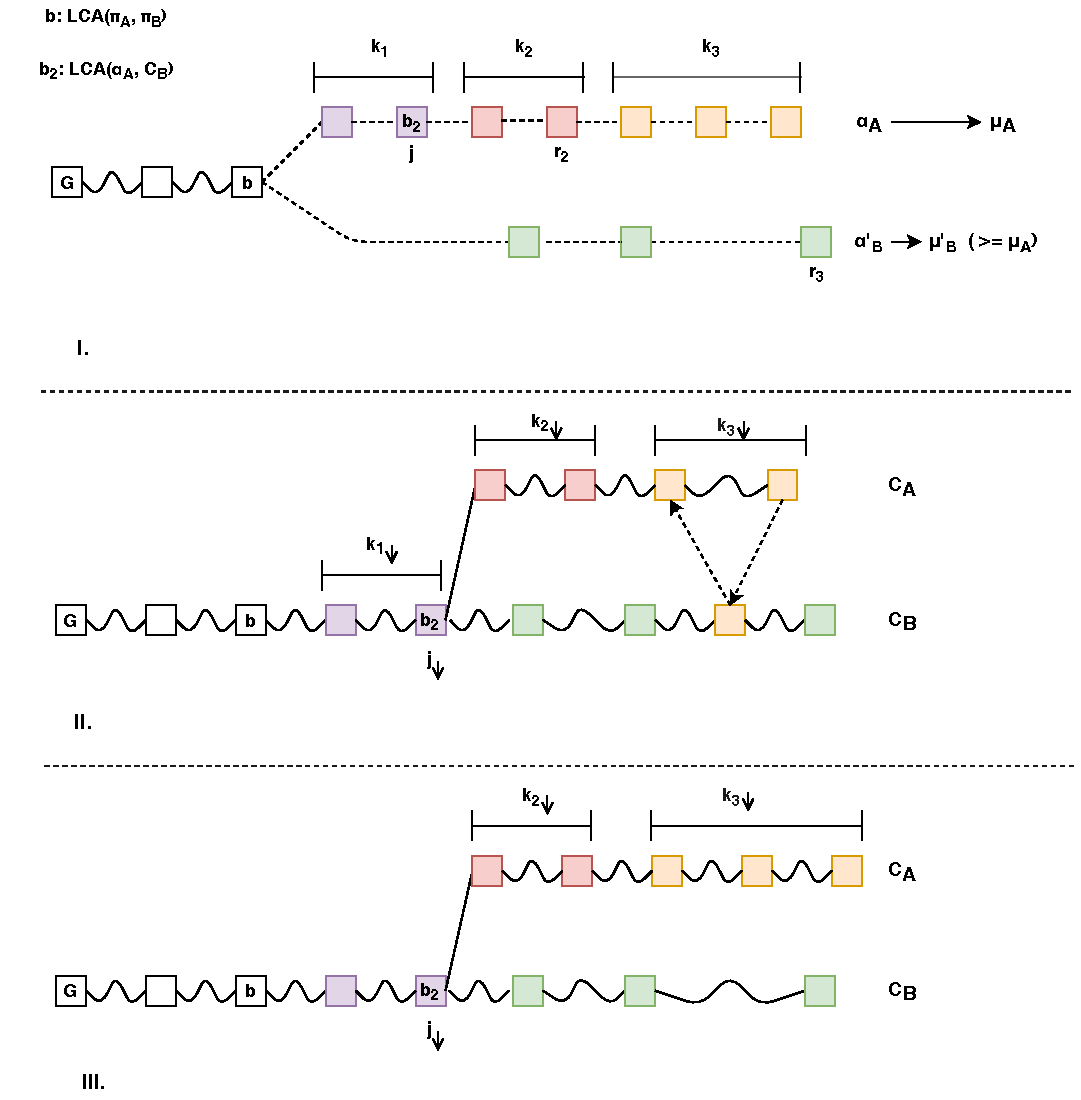
\includegraphics[scale=0.8]{figures/proof_velvet.pdf}
	\end{center}
	\caption{\textit{ Wavy lines imply one or more blocks. Dashed lines and arrows imply
	interlink pointers to superblocks. \textbf{I}: the three round sets in two competing
	proofs at different levels, \textbf{II}: the corresponding 0-level blocks implied by the two proofs,
	\textbf{III}: blocks participating in chain $\mathcal{C}_B$ and block set $\widetilde{\mathcal{C}}_\mathcal{A}$ from the verifier's perspective.}}	
    \label{fig:proof_velvet}
\end{figure}

From Corollary \ref{cor:adversarial_proof_scheme} we have that the adversarial proof 
consists of a smooth interlink subchain followed by a thorny interlink subchain. We will refer to the smooth part of $\alpha_\mathcal{A}$ as $\alpha^{\mathcal{S}}_\mathcal{A}$ and to the thorny part as $\alpha^{\mathcal{T}}_\mathcal{A}$.   

We will now show three successive claims under velvet fork conditions: First,
$\alpha^{\mathcal{S}}_\mathcal{A}$ and $\alpha'_B \downarrow$ are mostly
disjoint. Second, $a_A$ contains mostly adversarially generated blocks. And third,
the adversary is able to produce this $a_A$ with negligible probability.\\
Let $\alpha_A = k_1 + k_2 + k_3$ and let $k_1, k_2, k_3$ be as defined in the
following Claims.\\
Let round $r_1$ be the round when block $b$ is generated and round $r_2$ when block
$b_2 = LCA(\alpha_A, \alpha'_B\downarrow)$ is generated.\\

\textbf{Claim 1:} $\alpha^{\mathcal{S}}_\mathcal{A}$ and
$\alpha'_B\downarrow$ are mostly disjoint. Following the proof of Theorem 
\ref{thm:original_suffix_security} we conclude that 
$\vert \alpha^{\mathcal{S}}_\mathcal{A} \cap \alpha'_B\downarrow[1:] \vert \leq k_{1} = 2^{\mu'_B - \mu_A}$. 
In order to see this under the velvet fork conditions, first consider that the adversary behaves honestly for blocks in her proof generated between $b$ and $b_2$. This means that if $b_2$ was generated at round $r_{b_2}$ and $\alpha^{\mathcal{S}}_\mathcal{A}[-1]$ in round $r$, then $r \geq r_{b_2}$. In this case Claim 1 of
Theorem \ref{thm:original_suffix_security} applies directly. In the opposite case, the adversary includes a thorny block $b_t = \alpha^{\mathcal{T}}_{\mathcal{A}}[0]$ after $b$ and before $b_2$, thus the inequality still
holds and because of Lemma \ref{lemm:thorny_after_thorny} no more honestly generated blocks can be included
in $\alpha_A$ after $b_t$ and we can immediately proceed to Claim 3 of this proof.

We conclude that there are at least $\vert \alpha_A \vert - k_1$ blocks after
block $b$ in $\alpha_A$ which are not honestly generated blocks existing in
$\alpha'_B\downarrow$. In other words, there are $\vert \alpha_A \vert - k_1$
blocks after block $b$ in $\alpha_A$, which are either adversarially generated
existing in $\alpha_B\downarrow$ either don't belong in $\alpha_B\downarrow$.\\

\textbf{Claim 2.} 
At least $k_3$ superblocks of $\alpha_A$ are adversarially generated. Just as
the proof of Theorem \ref{thm:original_suffix_security} and using a similar notation, because of the Common Prefix
property on parameter $k_{2\downarrow}$, $\alpha_A[k_{1}+k_{2}:]$ could contain
no honestly generated blocks. In order to see this for the velvet fork conditions
let's again consider the case that the adversary behaves honestly for the first
$(k_1 + k_2)$ blocks of her proof in which case Claim 2 of Theorem 
\ref{thm:original_suffix_security} is immediately applied. In the opposite case,
the adversary includes in her proof a
thorny block at some earlier point. Again, because of Lemma 
\ref{lemm:thorny_after_thorny} the inequality still holds and no more
honestly generated blocks can be included in $\alpha_A$, so we can proceed to Claim 3
of this proof.\\

%\begin{figure}[h!]
%	\begin{center}
%		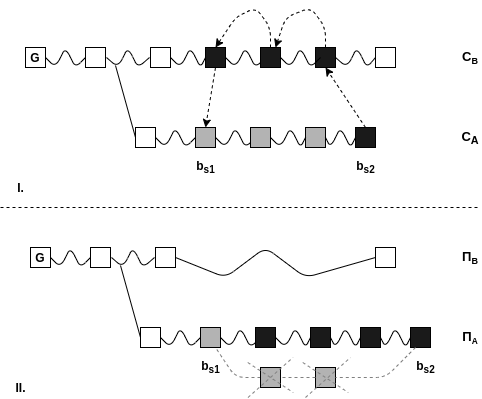
\includegraphics[scale=0.5]{figures/exclude.png}
%	\end{center}
%	\caption{\textit{ Wavy lines imply one or more blocks. Dashed arrows imply interlink 
%pointers to superblocks. Adversarially generated blocks are colored black. Grey colored 
%blocks may be honestly or adversarially generated. \textbf{I}: the 0-level chains, 
%\textbf{II}: the corresponding proof chains; some blocks generated in $C_A$ are excluded 
%from proof $\pi_A$ in favor of the sewed blocks from $C_B$.}}
%	\label{fig:exclude}
%\end{figure}

\textbf{Claim 3.} The adversary may submit a suffix proof such that $\alpha_A \geq \alpha_B$
with negligible probability.
%%% @TODO: make formal arguments
As argued aerlier the last $k_3$ blocks included in $\alpha_A$ are all adversarially generated. In the worst case  all $k_3 $ blocks
are sewed from $C_B$. This is the worst case scenario since each adversarially
generated block in $C_B$ may have dropped one honest block out of the chain
because of selfish mining. Considering this scenario, because of the strengthened
Honest Majority Assumption for $(1/3)$-bounded adversary, Theorem 3 for Chain
Quality guarantees that the majority of the blocks in $C_B$ was computed by
honest parties, thus the honestly generated blocks in $C_B$ for the same round
set sum to more amount of hashing power.\\
From all the above Claims we have that:\\
In the first round set, because of the common underlying chain:
\begin{equation} \label{eq_v_round_set_1}
2^{\mu_A} \vert \alpha_A^{k_1} \vert \leq 2^{\mu'_B} \vert \alpha'{_B^{k_1}} \vert
\end{equation}
Because of the adoption by an honest party of chain $C_B$ at a later round $r_3$, we
have for the second round set:
\begin{equation} \label{eq_v_round_set_2}
2^{\mu_A} \vert \alpha_A^{k_2} \vert \leq 2^{\mu'_B} \vert \alpha'{_B^{k_2}} \vert
\end{equation}
In the third round set, because of good Chain Quality under the strengthened Honest
Majority Assumption and Theorem 3 we have:
\begin{equation} \label{eq_v_round_set_3}
2^{\mu_A} \vert \alpha_A^{k_3} \vert < 2^{\mu'_B} \vert \alpha'{_B^{k_3}} \vert
\end{equation}
Consequently we have:

\begin{equation} \label{eq_v_all_round_sets}
2^{\mu_A} \vert \alpha_A \vert < 2^{\mu'_B} \vert \alpha'{_B} \vert
\end{equation}
